


\begin{figure}[t]
    \begin{minipage}[b]{.6\linewidth}
        \centering
        \small
        \renewcommand{\arraystretch}{0.2}
        \setlength{\tabcolsep}{0.3pt}
        \begin{tabular}{ccccccc}
           \rotatebox[origin=c]{-90}{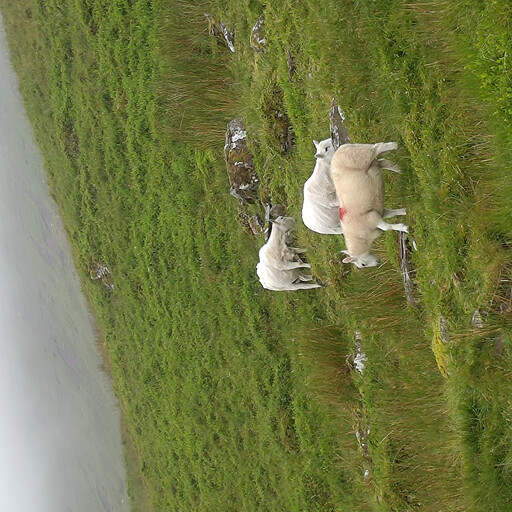
\includegraphics[width=0.32\linewidth]{images/evolution_cosine_u1/P_20240709_135144.jpg_croped.lr.jpg}} & 
          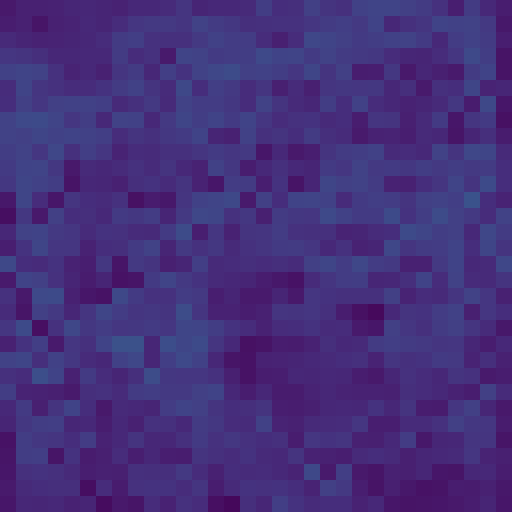
\includegraphics[width=0.32\linewidth]{images/evolution_cosine_u1/P_20240709_135144.jpg_iter199999_512_seed0.png} & 
          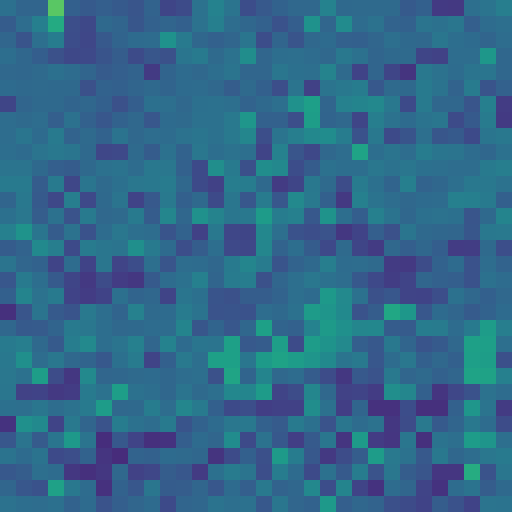
\includegraphics[width=0.32\linewidth]{images/evolution_cosine_u1/P_20240709_135144.jpg_iter999999_512_seed0.png} 
          \\
           \rotatebox[origin=c]{-90}{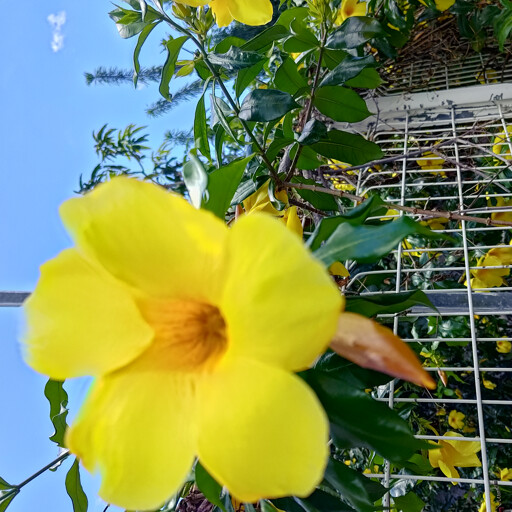
\includegraphics[width=0.32\linewidth]{images/evolution_cosine_u1/P_20250105_134132.jpg_croped.lr.jpg}} & 
          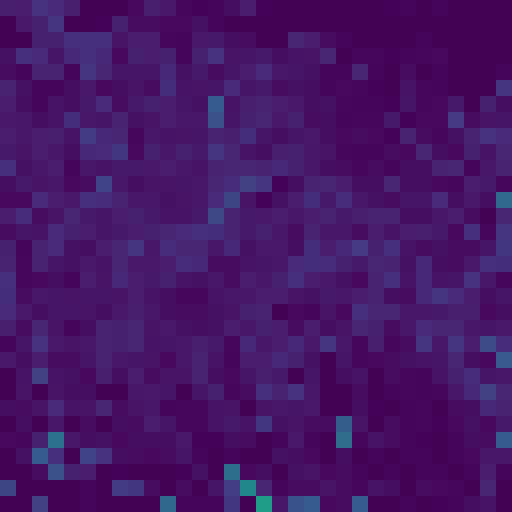
\includegraphics[width=0.32\linewidth]{images/evolution_cosine_u1/P_20250105_134132.jpg_iter199999_512_seed0.png} & 
          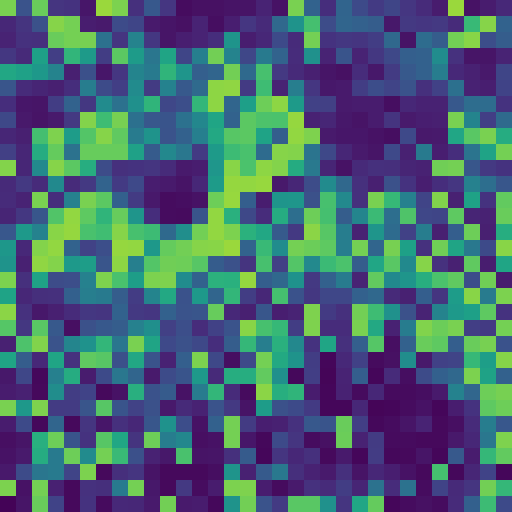
\includegraphics[width=0.32\linewidth]{images/evolution_cosine_u1/P_20250105_134132.jpg_iter999999_512_seed0.png} 
          \\[0.5em]
          Image & 200k & 1M
        \end{tabular}
        
        \subcaption{Cosine similarities between the CLS and output patches.}
        \label{fig:evolution-cls}
    \end{minipage}%
    \hfill
    \begin{minipage}[b]{.4\linewidth}
        \centering
        \refstepcounter{subfigure}  %
        \label{fig:evolution-cls-g}
        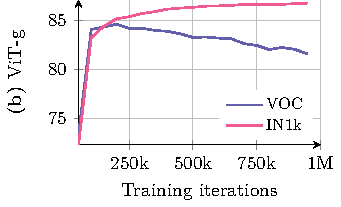
\includegraphics{figures/tikz/gram_evolution_pregram_g.pdf}%

        \vspace{0.35em}
        \refstepcounter{subfigure}  %
        \label{fig:evolution-cls-7B}
        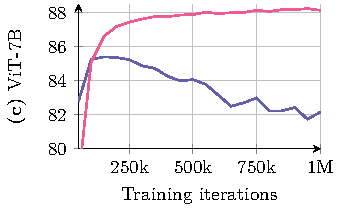
\includegraphics{figures/tikz/gram_evolution_pregram_7b.pdf}%
        \vspace{0.35em}
    \end{minipage}%
    
    \caption{Evolution of the cosine similarities (a) and of the accuracy on ImageNet1k linear (IN1k) and segmentation on VOC for ViT-g (b) and ViT-7B (c). We observe that the segmentation performance is maximal when the cosine similarities between the patch tokens and the class tokens are low. As training progresses, these similarities increase and the performance on dense tasks decreases.}
    \label{fig:gram:evolution}
\end{figure}

\section[Gram: A Regularization for Dense Features]{\Gramname: A Regularization for Dense Features}
\label{sec:gram}

To fully leverage the benefits of large-scale training, we aim to train the 7B model for an extended duration, with the notion that it could potentially train indefinitely. As expected, prolonged training leads to improvements on global benchmarks. However, as training progresses, the performance degrades on dense tasks (\cref{fig:evolution-cls-g,fig:evolution-cls-7B}). 
This phenomenon, which is due to the emergence of patch-level inconsistencies in feature representations, undermines the interest behind extended training.\footnote{%
We also observed different types of outliers appearing with continued training; we provide a discussion in \cref{app:sec:artifacts}.
} 
In this section, we first analyze the loss of patch-level consistency, then propose a new objective to mitigate it, called \emph{\gramname}. 
We finally discuss the impact of our approach on both training stability and model performance.


\subsection{Loss of Patch-Level Consistency Over Training}





\begin{figure}[t]
    \centering
    \small
    \renewcommand{\arraystretch}{0.2}
    \setlength{\tabcolsep}{0.3pt}
    \begin{tabular}{@{}ccccccc@{}}
       \rotatebox[origin=c]{-90}{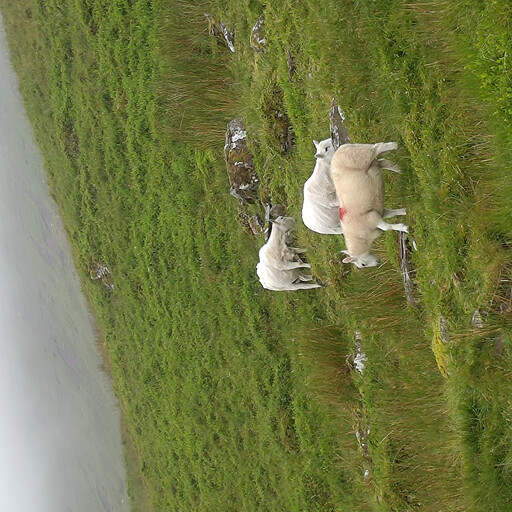
\includegraphics[width=0.165\linewidth]{images/evolution_cosine_u1/P_20240709_135144.jpg_croped.lr.jpg}} & 
      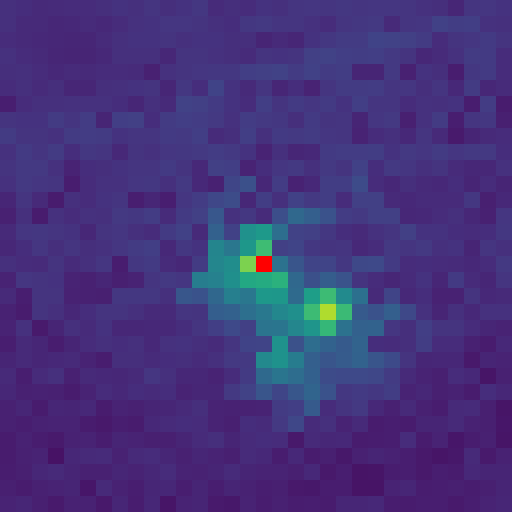
\includegraphics[width=0.165\linewidth]{images/evolution_cosine_u1/P_20240709_135144.jpg_iter199999_512.png} & 
      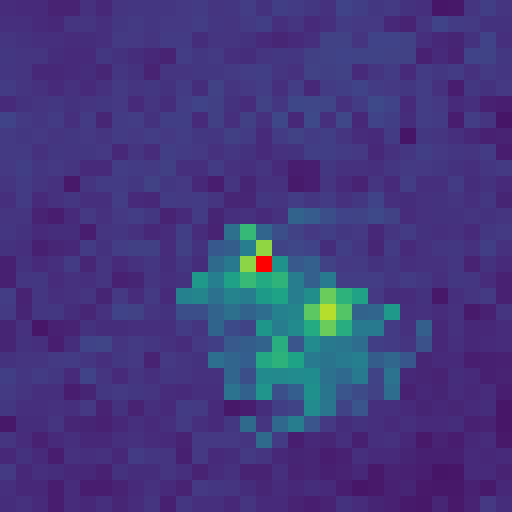
\includegraphics[width=0.165\linewidth]{images/evolution_cosine_u1/P_20240709_135144.jpg_iter399999_512.png} & 
      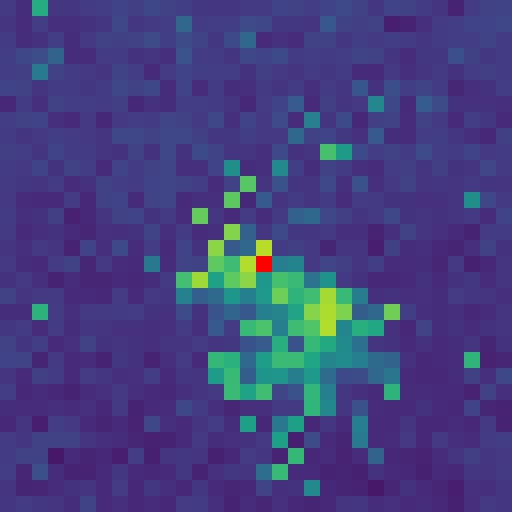
\includegraphics[width=0.165\linewidth]{images/evolution_cosine_u1/P_20240709_135144.jpg_iter599999_512.png} & 
      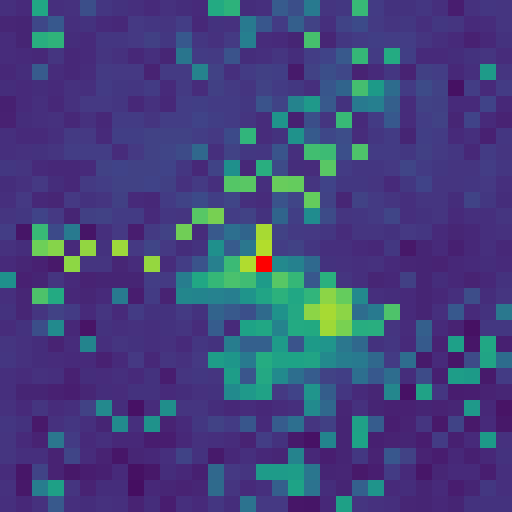
\includegraphics[width=0.165\linewidth]{images/evolution_cosine_u1/P_20240709_135144.jpg_iter799999_512.png} & 
      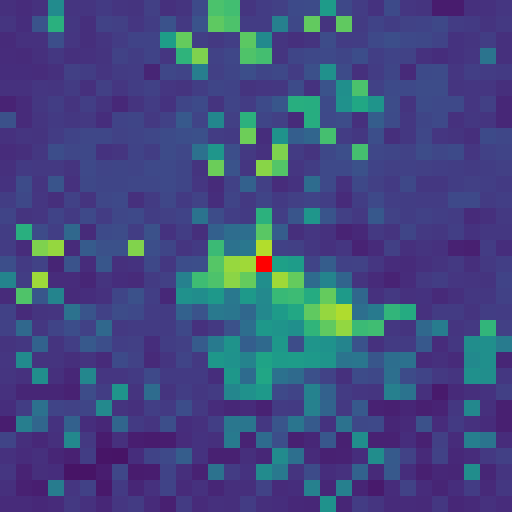
\includegraphics[width=0.165\linewidth]{images/evolution_cosine_u1/P_20240709_135144.jpg_iter999999_512.png} 
      \\
       \rotatebox[origin=c]{-90}{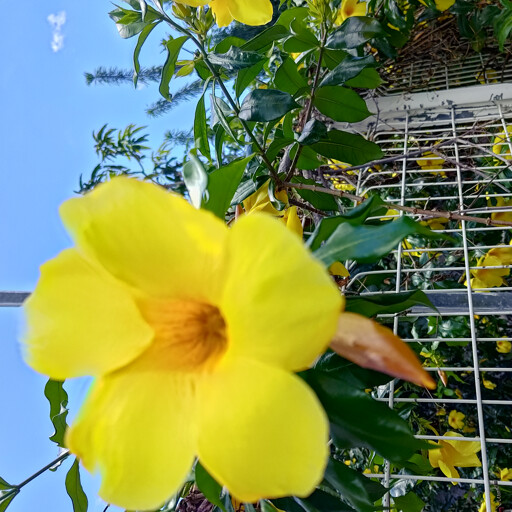
\includegraphics[width=0.165\linewidth]{images/evolution_cosine_u1/P_20250105_134132.jpg_croped.lr.jpg}} & 
      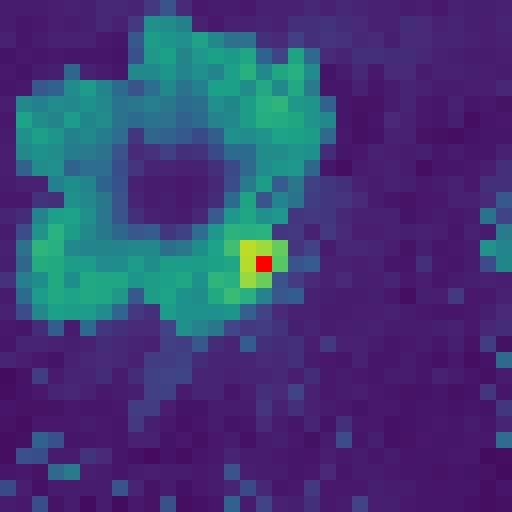
\includegraphics[width=0.165\linewidth]{images/evolution_cosine_u1/P_20250105_134132.jpg_iter199999_512.png} & 
      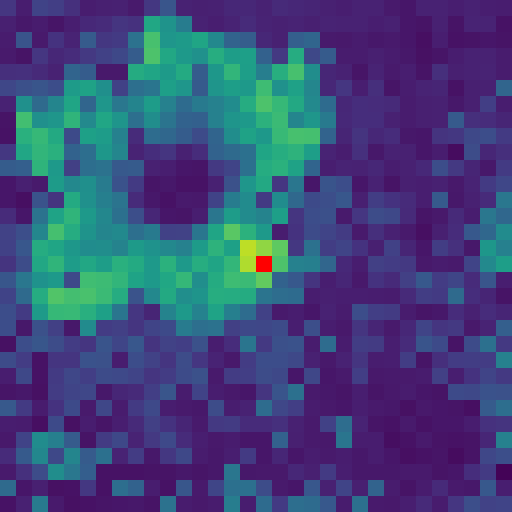
\includegraphics[width=0.165\linewidth]{images/evolution_cosine_u1/P_20250105_134132.jpg_iter399999_512.png} & 
      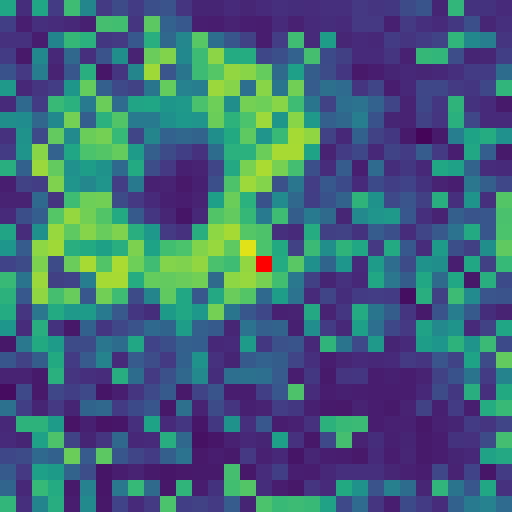
\includegraphics[width=0.165\linewidth]{images/evolution_cosine_u1/P_20250105_134132.jpg_iter599999_512.png} & 
      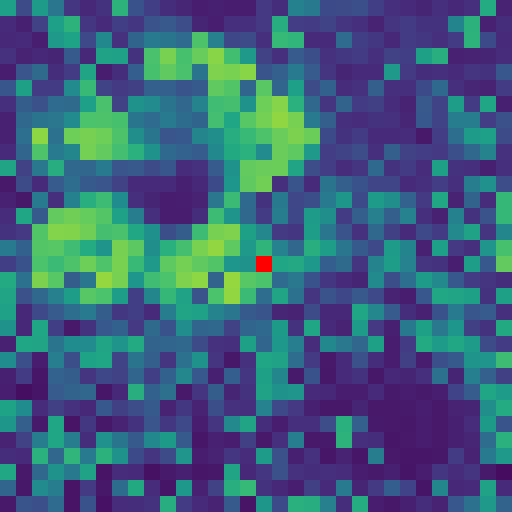
\includegraphics[width=0.165\linewidth]{images/evolution_cosine_u1/P_20250105_134132.jpg_iter799999_512.png} & 
      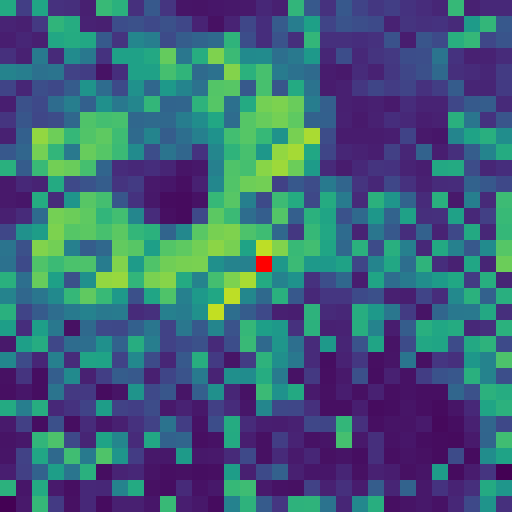
\includegraphics[width=0.165\linewidth]{images/evolution_cosine_u1/P_20250105_134132.jpg_iter999999_512.png} 
      \\[0.5em]
      Image & 200k & 400k & 600k & 800k & 1M \\
    \end{tabular}
    \caption{
     Evolution of the cosine similarity between the patch noted in red and all other patches.
     As training progresses, the features produced by the model become less localized and the similarity maps become noisier.
    }
    \label{fig:evolution-cosines}
\end{figure}

During extended training, we observe consistent improvements in global metrics but a notable decline in performance on dense prediction tasks. 
This behavior was previously observed, to a lesser extent, during the training of DINOv2, and also discussed in the scaling effort of \citet{fan2025scaling}.
However, to the best of our knowledge, it remains unresolved to date.
We illustrate the phenomenon in \cref{fig:evolution-cls-g,fig:evolution-cls-7B}, which present the performance of the model across iterations on both image classification and segmentation tasks. 
For classification, we train a linear classifier on ImageNet-1k using the CLS token and report top-1 accuracy. 
For segmentation, we train a linear layer on patch features extracted from Pascal VOC and report mean Intersection over Union (mIoU). 
We observe that both for the ViT-g and the ViT-7B, the classification accuracy monotonically improves throughout training. 
However, segmentation performance declines in both cases after approximately 200k iterations, falling below its early levels in the case of the ViT-7B.

To better understand this degradation, we analyze the quality of patch features by visualizing cosine similarities between patches. \cref{fig:evolution-cosines} shows the cosine similarity maps between the backbone’s output patch features and a reference patch (highlighted in red). At 200k iterations, the similarity maps are smooth and well-localized, indicating consistent patch-level representations. However, by 600k iterations and beyond, the maps degrade substantially,  with an increasing number of irrelevant patches with high similarity to the reference patch. 
This loss of patch-level consistency correlates with the drop in dense task performance.

These patch-level irregularities differ from the high-norm patch outliers described in \citet{darcet2024vision}. 
Specifically, with the integration of register tokens, patch norms remain stable throughout training. However, we notice that the cosine similarity between the CLS token and the patch outputs gradually increases during training. This is expected, yet it means that the locality of the patch features diminishes. We visualize this phenomenon in \cref{fig:evolution-cls}, which depicts the cosine maps at 200k and 1M iterations. 
In order to mitigate the drop on dense tasks, we propose a new objective specifically designed to regularize the patch features and ensure a good patch-level consistency, while preserving high global performance.












\subsection[Gram Objective]{\Gramname Objective}

\begin{figure}[t]
    \centering
    \begin{subfigure}{0.32\linewidth} 
        \centering
        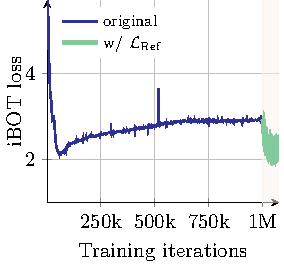
\includegraphics{figures/tikz/gram_losses_ibot.pdf}
        \caption{iBOT loss}
    \end{subfigure}
    \hfill
    \begin{subfigure}{0.32\linewidth} 
        \centering
        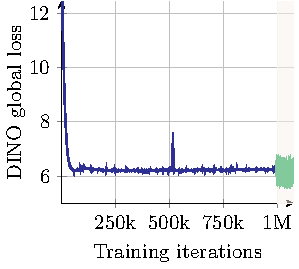
\includegraphics{figures/tikz/gram_losses_dino.pdf}
        \caption{DINO global loss}
    \end{subfigure}
    \hfill
    \begin{subfigure}{0.32\linewidth} 
        \centering
        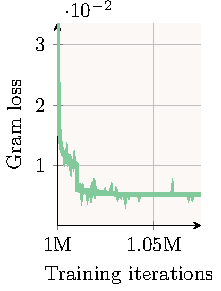
\includegraphics{figures/tikz/gram_losses_gram.pdf}
        \caption{Gram loss}
    \end{subfigure}
    \caption{Evolution trough the training iterations of the patch-level iBOT loss, the global loss DINO (applied to the global crops) and the newly introduced Gram loss. We \colorbox{White!90!Tan}{highlight} the iterations of the refinement step $\mathcal{L}_\mathrm{Ref}$ which uses the Gram objective. }
    \label{fig:losses}
\end{figure}

Throughout our experiments, we have identified a relative independence between learning strong discriminative features and maintaining local consistency, as observed in the lack of correlation between global and dense performance. 
While combining the global DINO loss with the local iBOT loss has begun to address this issue, we observe that the balance is unstable, with global representation dominating as training progresses.
Building on this insight, we propose a novel solution that explicitly leverages this independence. 

We introduce a new objective which mitigates the degradation of patch-level consistency by enforcing the quality of the patch-level consistency, without impacting the features themselves.
This new loss function %
operates on the Gram matrix: the matrix of all pairwise dot products of patch features in an image.
We want to push the Gram matrix of the student towards that of an earlier model, referred to as the \emph{Gram teacher}.
We select the Gram teacher by taking an early iteration of the teacher network, which exhibits superior dense properties. 
By operating on the Gram matrix rather than the feature themselves, the local features are free to move, provided the structure of similarities remains the same.
Suppose we have an image composed of $P$ patches, and a network that operates in dimension $d$.
Let us denote by $\mathbf{X}_S$ (respectively $\mathbf{X}_{G}$) the $P \times d$ matrix of $\mathbf{L}_2$-normalized local features of the student (respectively the Gram teacher).
We define the loss $\mathcal{L}_{\text{Gram}}$ as follows: 
\begin{equation}
  \mathcal{L}_{\text{Gram}} = \left \| \mathbf{X}_{S} \cdot \mathbf{X}_{S}^\top - \mathbf{X}_{G} \cdot \mathbf{X}_{G}^\top  \right \|_\text{F}^2.
  \label{eq:gram-loss}
\end{equation}

We only compute this loss on the global crops.
Even though it can be applied early on during the training, for efficiency, we start only after $1$M iterations.
Interestingly, we observe that the late application of $\mathcal{L}_{\text{Gram}}$ still manages to ``repair'' very degraded local features.
In order to further improve performance, we update the Gram teacher every 10k iterations at which the Gram teacher becomes identical to the main EMA teacher.  
We call this second step of training the \emph{refinement step}, which optimizes the objective $\mathcal{L}_\mathrm{Ref}$, with 
\begin{equation}
    \mathcal{L}_\mathrm{Ref} = w_{\mathrm{D}}\mathcal{L_{\mathrm{DINO}}} + \mathcal{L}_{\mathrm{iBOT}} + w_{\mathrm{DK}}\mathcal{L}_{\mathrm{DKoleo}} + w_{\mathrm{Gram}}\mathcal{L}_{\mathrm{Gram}}.
\end{equation}
We visualize the evolution of different losses in \cref{fig:losses} and observe that applying the Gram objective significantly influences the iBOT loss, causing it to decrease more rapidly. 
This suggests that the stability introduced by the stable Gram teacher positively impacts the iBOT objective. In contrast, the Gram objective does not have a significant effect on the DINO losses. 
This observation implies that the Gram and iBOT objectives impact the features in a similar way, whereas the DINO losses affect them differently.

Regarding performance, we observe the impact of the new loss is almost immediate. 
As shown in \cref{fig:evolution-gram}, incorporating \gramname leads to significant improvements on dense tasks within the first 10k iterations. 
We also see notable gains on the ADE20k benchmark following the Gram teacher updates. 
Additionally, longer training further benefits performance on the ObjectNet benchmark and other global benchmarks show mild impact from the new loss.

\begin{figure}[t]
    \centering
    \begin{subfigure}{0.32\linewidth} 
        \centering
        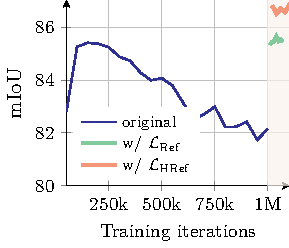
\includegraphics{figures/tikz/gram_evolution_voc.pdf}
        \caption{VOC}
    \end{subfigure}
    \hfill
    \begin{subfigure}{0.32\linewidth} 
      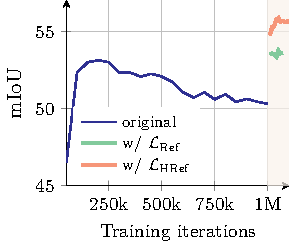
\includegraphics{figures/tikz/gram_evolution_ade20k.pdf}
        \caption{ADE20k}
    \end{subfigure}
    \hfill
    \begin{subfigure}{0.32\linewidth} 
      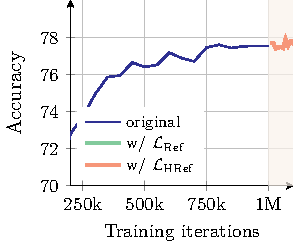
\includegraphics{figures/tikz/gram_evolution_objectnet.pdf}
        \caption{ObjectNet}
    \end{subfigure}    
    \caption{
        Evolution of the results on different benchmarks after applying our proposed \emph{\gramname} method.
        We visualize results when continuing the original training with our refinement step, noted `$\mathcal{L}_\mathrm{Ref}$'.
        We also plot results obtained when using higher-resolution features for the Gram objective as introduced in following \cref{sec:high-res-feats} and noted `$\mathcal{L}_\mathrm{HRef}$'.
        We \colorbox{White!90!Tan}{highlight} the iterations which use the Gram objective. 
    }
    \label{fig:evolution-gram}
\end{figure}

\subsection{Leveraging Higher-Resolution Features}
\label{sec:high-res-feats}

Recent work shows that a weighted average of patch features can yield stronger local representations by smoothing outlier patches and enhancing patch-level consistency~\citep{wysoczanska2023clipdino}. 
On the other hand, feeding higher-resolution images into the backbone produces finer and more detailed feature maps. 
We leverage the benefits of both observations to compute high-quality features for Gram teacher.
Specifically, we first input images at twice the normal resolution into the Gram teacher, then $2\times$ down-sample the resulting feature maps with the bicubic interpolation to achieve the desired smooth feature maps that match the size of the student output.
\cref{fig:gram-resolutions} visualizes the Gram matrices of patch features obtained with images at resolutions 256 and 512, as well as those obtained after $2\times$ down-sampling features from the 512-resolution (denoted as ‘downsamp.’). We observe that the superior patch-level consistency in the higher-resolution features is preserved through down-sampling, resulting in smoother and more coherent patch-level representations. As a side note, our model can seamlessly process images at varying resolutions without requiring adaptation, thanks to the adoption of Rotary Positional Embeddings (RoPE) introduced by \citet{su2024roformer}.


We compute the Gram matrix of the down-sampled features and use it to replace $\mathbf{X}_{G}$ in the objective $\mathcal{L_{\mathrm{Gram}}}$. We note the new resulting refinement objective as $\mathcal{L}_\mathrm{HRef}$. 
This approach enables the Gram objective to effectively distill the improved patch consistency of smoothed high-resolution features into the student model.
As shown in \cref{fig:evolution-gram} and \cref{tab:gram-teacher-res}, this distillation translates into better predictions on dense tasks, yielding additional gains on top of the benefit brought by $\mathcal{L}_\mathrm{Ref}$ (+2 mIoU on ADE20k).
We also ablate the choice of Gram teacher in \cref{tab:gram-teacher-res}. 
Interestingly, choosing the Gram teacher from 100k or 200k does not significantly impact the results,
but using a much later Gram teacher (1M iterations) is detrimental because the patch-level consistency of such a teacher is inferior. 

Finally, we qualitatively illustrate the effect of Gram anchoring to patch-level consistency in \cref{fig:gram-matrices-comp} which visualizes the Gram matrices patch features obtained with the initial training and high-resolution \gramname refinement.
We observe great improvements in feature correlations that our high-resolution refinement procedure brings about.

\begin{figure}[t]
    \begin{subfigure}{.495\linewidth}    
        \centering
        \renewcommand{\arraystretch}{0.2}
        \setlength{\tabcolsep}{0.5pt}
        \begin{tabular}{cccc}
        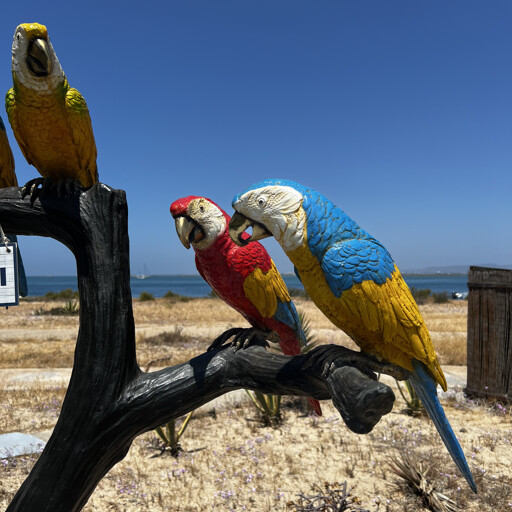
\includegraphics[height=0.23\textwidth]{images/gram/comparison_res/IMG_0877.HEIC_croped.lr.jpg} &
            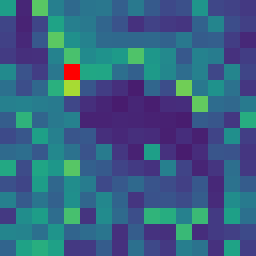
\includegraphics[height=0.23\textwidth]{images/gram/comparison_res/IMG_0877.HEIC_256.png} & 
            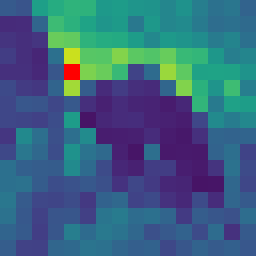
\includegraphics[height=0.23\textwidth]{images/gram/comparison_res/IMG_0877.HEIC_512to256.png} & 
            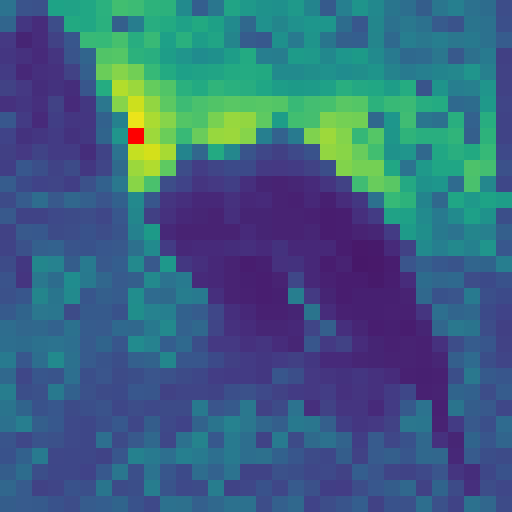
\includegraphics[height=0.23\textwidth]{images/gram/comparison_res/IMG_0877.HEIC_512.png} \\
            \rotatebox[origin=c]{-90}{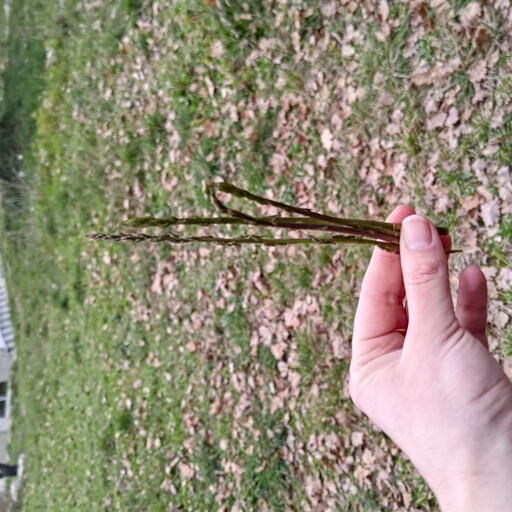
\includegraphics[height=0.23\textwidth]{images/gram/comparison_res/IMG_20250720_075113.jpg_croped.lr.jpg}} &
            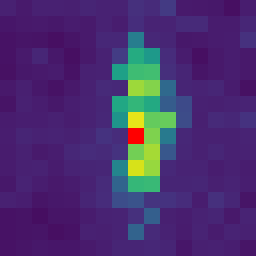
\includegraphics[height=0.23\textwidth]{images/gram/comparison_res/IMG_20250720_075113.jpg_256.png} & 
            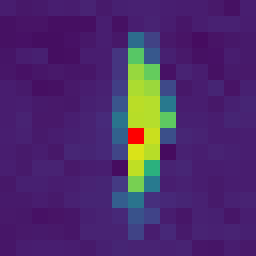
\includegraphics[height=0.23\textwidth]{images/gram/comparison_res/IMG_20250720_075113.jpg_512to256.png} & 
            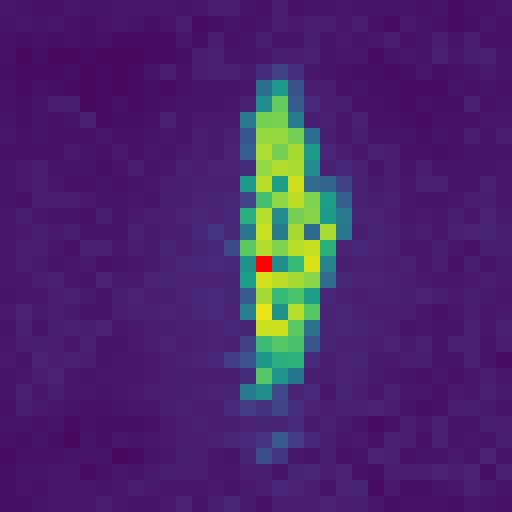
\includegraphics[height=0.23\textwidth]{images/gram/comparison_res/IMG_20250720_075113.jpg_512.png} \\\\
            Input &  $256$ &  Downsamp. &  $512$
        \end{tabular}
        \caption{Gram matrices at different input resolutions.}
        \label{fig:gram-resolutions}
    \end{subfigure}   
    \hfill 
    \begin{subfigure}[b]{.495\linewidth}
        \centering
        \small
        \setlength{\tabcolsep}{5pt}
        \begin{tabular}{@{}lcc  ccc@{}}
          \toprule
           & Teacher & Res.  &   IN1k   & ADE  & NYU \\
          Method & Iteration &&  Linear & mIoU & RMSE \\
          \midrule
          Baseline & --- & --- &          \bf 88.2 & 50.3 & 0.307 \\
          GRAM &          200k & $\times$1 & 88.0  & 53.6 & 0.285 \\
          GRAM &          200k & $\times$2 & 88.0 & \bf 55.7 & \bf 0.281 \\
          GRAM &          100k & $\times$2 & 87.9 & \bf 55.7 & 0.284 \\
          GRAM & \phantom{00}1M& $\times$2 & 88.1 & 54.9 & 0.290 \\
          \bottomrule
        \end{tabular}
        \vspace{1.5em}
        \caption{
          Ablation of Gram teachers and resolutions.
        }
        \label{tab:gram-teacher-res}
    \end{subfigure}
    \caption{Quantitative and qualitative study of the impact of high-resolution Gram. We show (a) the improved cosine maps after down-sampling the high-resolution maps into smaller ones, and (b) the quantitative improvements brought by varying the training iteration and the resolution of the Gram teacher.
    }
    \label{fig:gram}
\end{figure}

\begin{figure}[t]
    \centering
    \renewcommand{\arraystretch}{0.2}
    \setlength{\tabcolsep}{0.2pt}
    \begin{tabular}{@{}cccccc@{}}
    \raisebox{40pt}{\rotatebox[origin=c]{90}{original}} & 
    \rotatebox[origin=c]{-90}{
\includegraphics[width=0.19\textwidth]{images/gram/comparison_w_wo/P_20250105_134132.jpg_croped.lr.jpg}} & 
    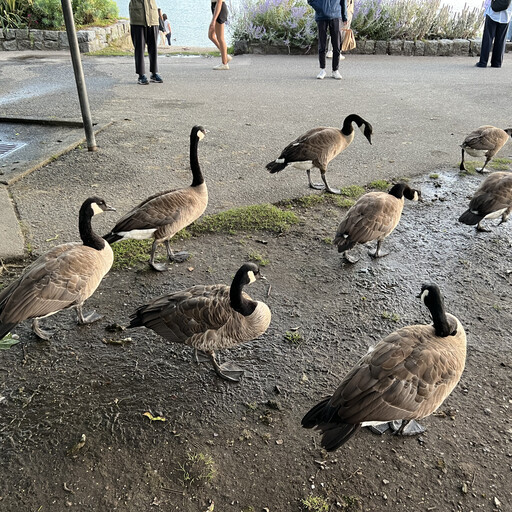
\includegraphics[width=0.19\textwidth]{images/gram/comparison_w_wo/IMG_3727.HEIC_croped.lr.jpg} & 
    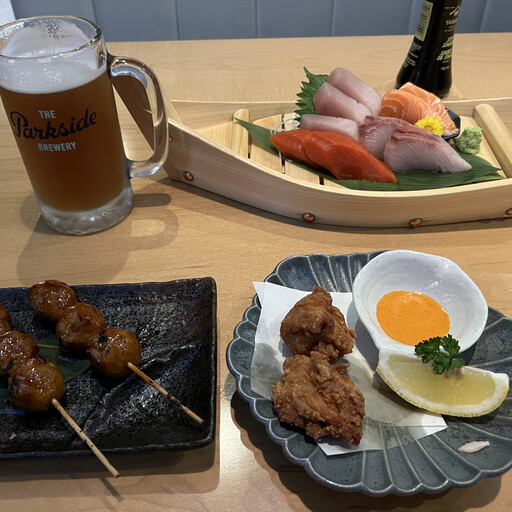
\includegraphics[width=0.19\textwidth]{images/gram/comparison_w_wo/IMG_3730.HEIC_croped.lr.jpg} & 
    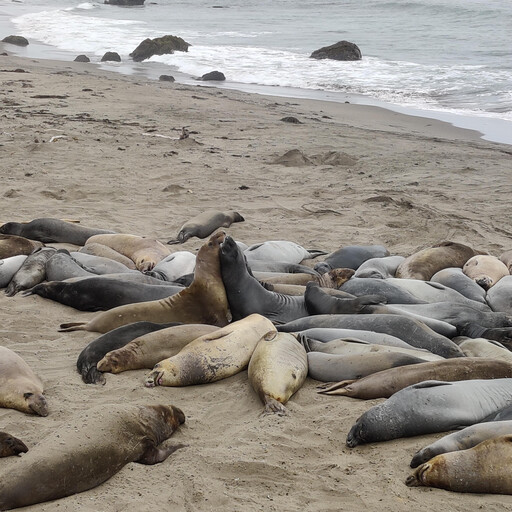
\includegraphics[width=0.19\textwidth]{images/gram/comparison_w_wo/IMG_20190618_192715.jpg_croped.lr.jpg} & 
    \rotatebox[origin=c]{-90}{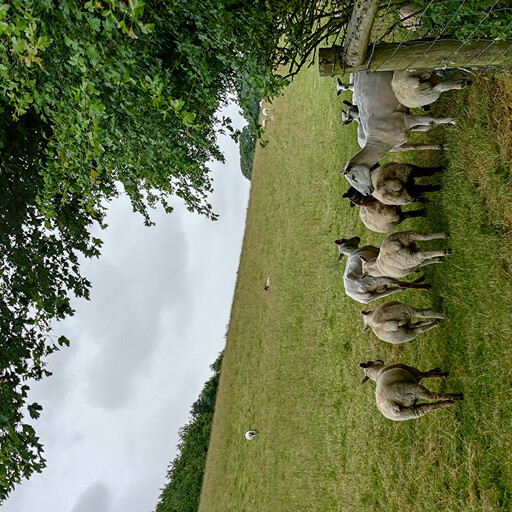
\includegraphics[width=0.19\textwidth]{images/gram/comparison_w_wo/P_20240705_151013.jpg_croped.lr.jpg}}
    
    \\
    \raisebox{40pt}{\rotatebox[origin=c]{90}{wo/ $\mathcal{L}_\mathrm{HRef}$}} & 
    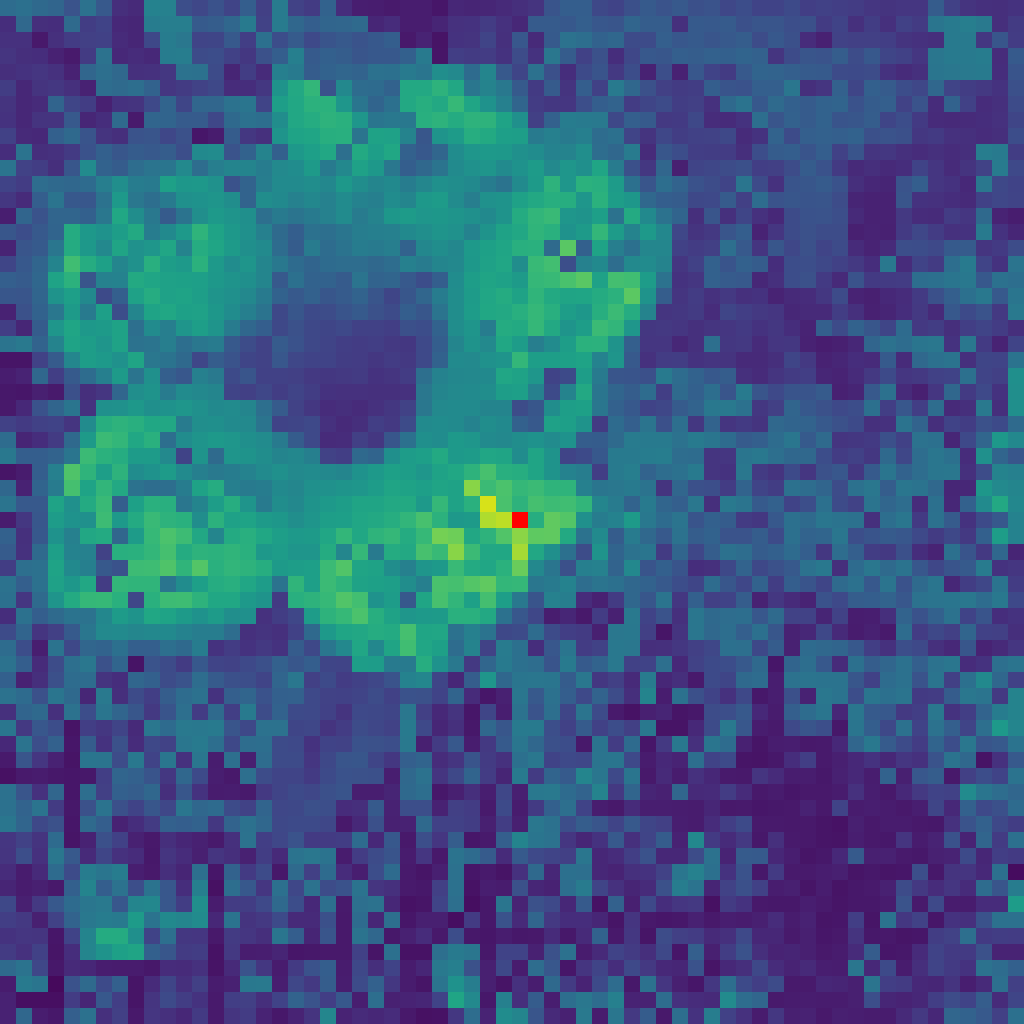
\includegraphics[width=0.19\textwidth]{images/gram/comparison_w_wo/P_20250105_134132.jpg_U1_iter999999_512_seed1.png} &
    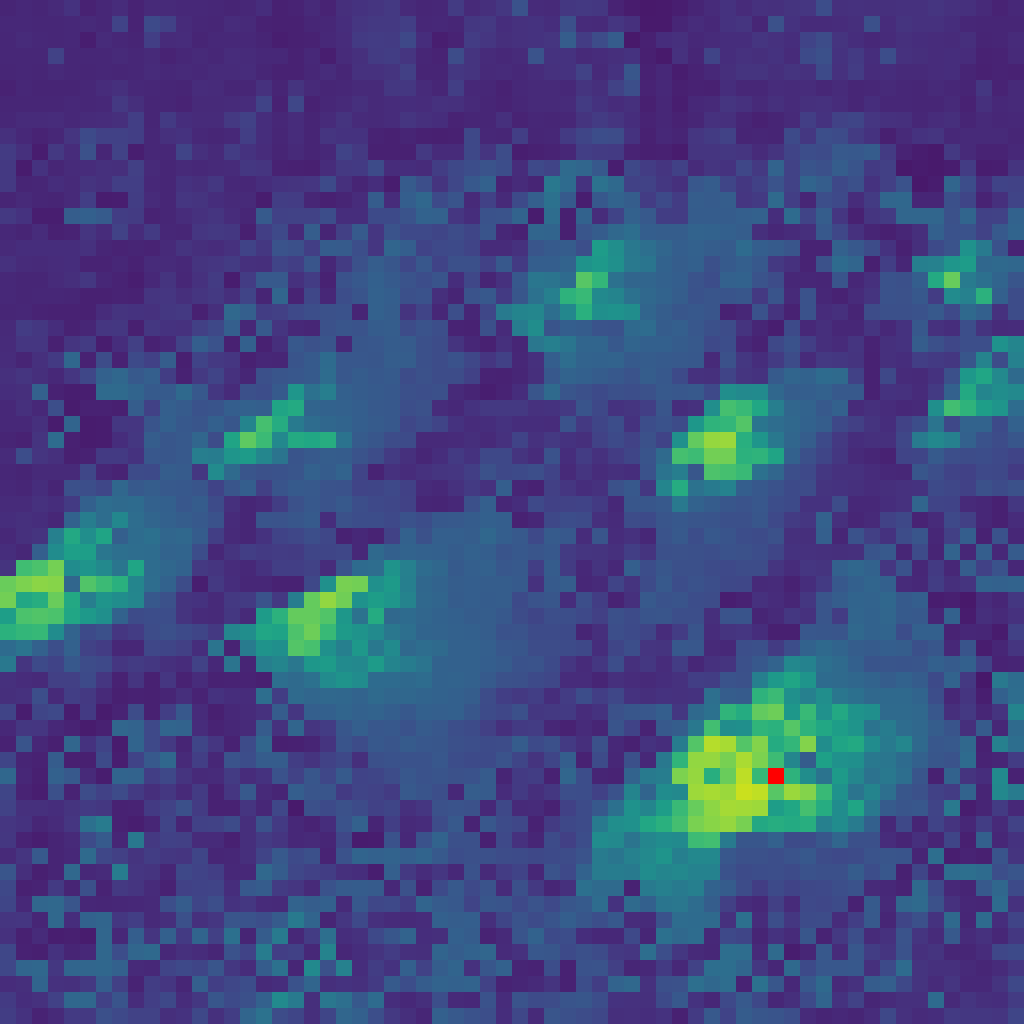
\includegraphics[width=0.19\textwidth]{images/gram/comparison_w_wo/IMG_3727.HEIC_U1_iter999999_512_seed5.png} & 
    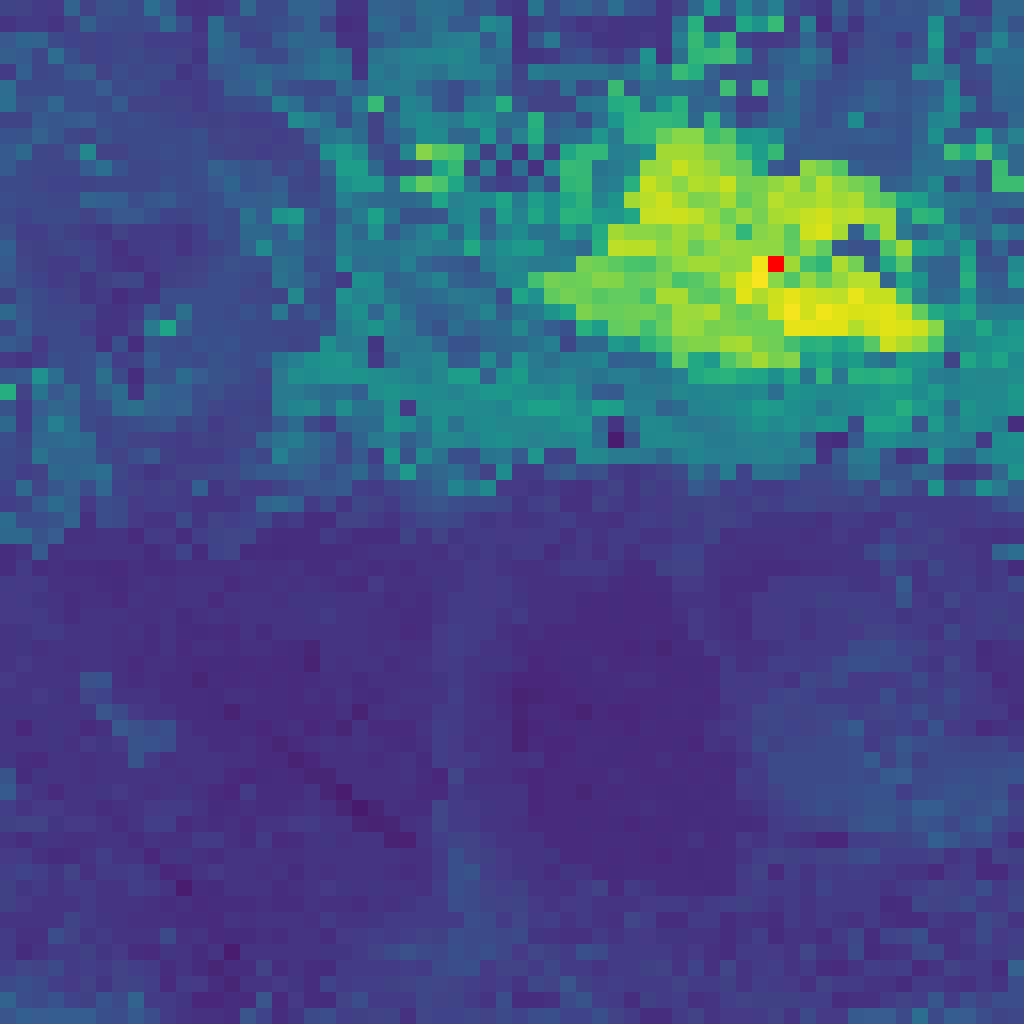
\includegraphics[width=0.19\textwidth]{images/gram/comparison_w_wo/IMG_3730.HEIC_U1_iter999999_512_seed3.png} &  
    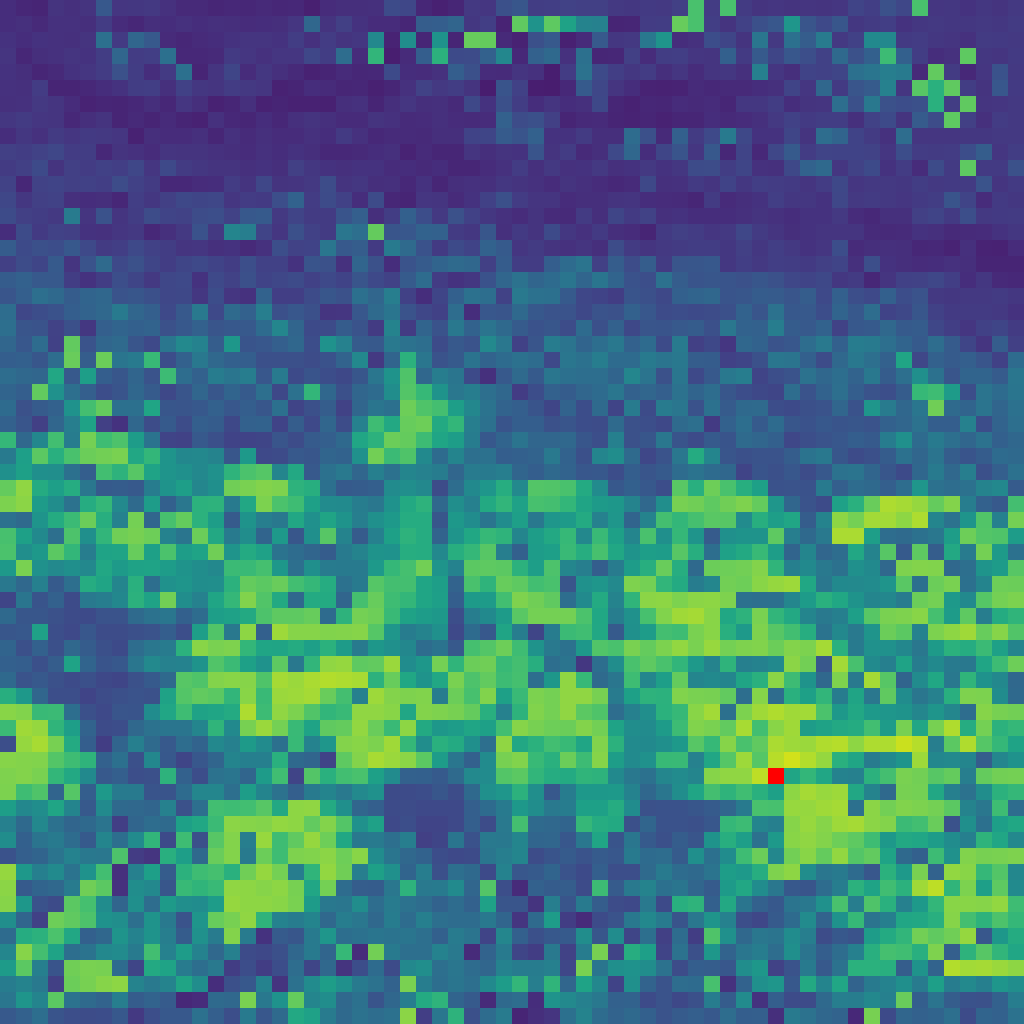
\includegraphics[width=0.19\textwidth]{images/gram/comparison_w_wo/IMG_20190618_192715.jpg_U1_iter999999_512_seed5.png} & 
    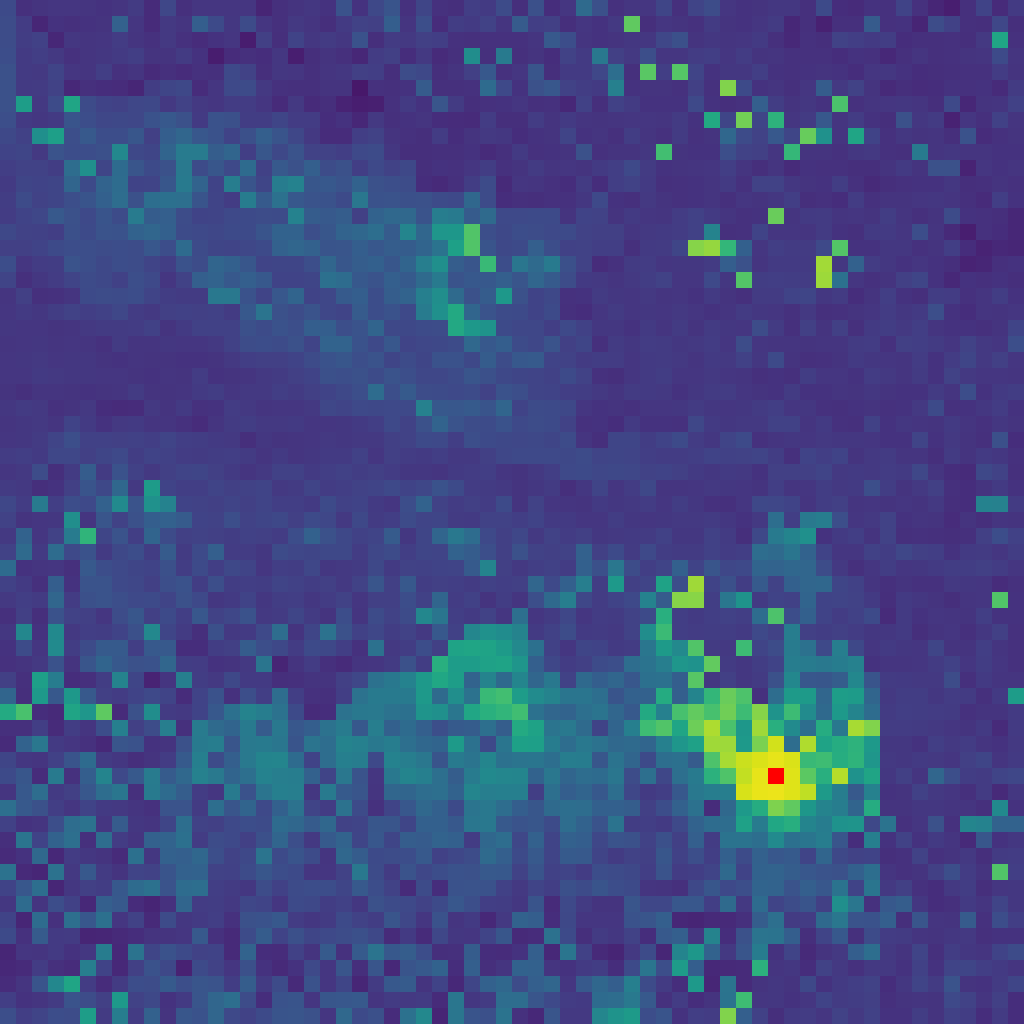
\includegraphics[width=0.19\textwidth]{images/gram/comparison_w_wo/P_20240705_151013.jpg_U1_iter999999_512_seed5.png}
    \\
    \raisebox{40pt}{\rotatebox[origin=c]{90}{w/ $\mathcal{L}_\mathrm{HRef}$}} & 
    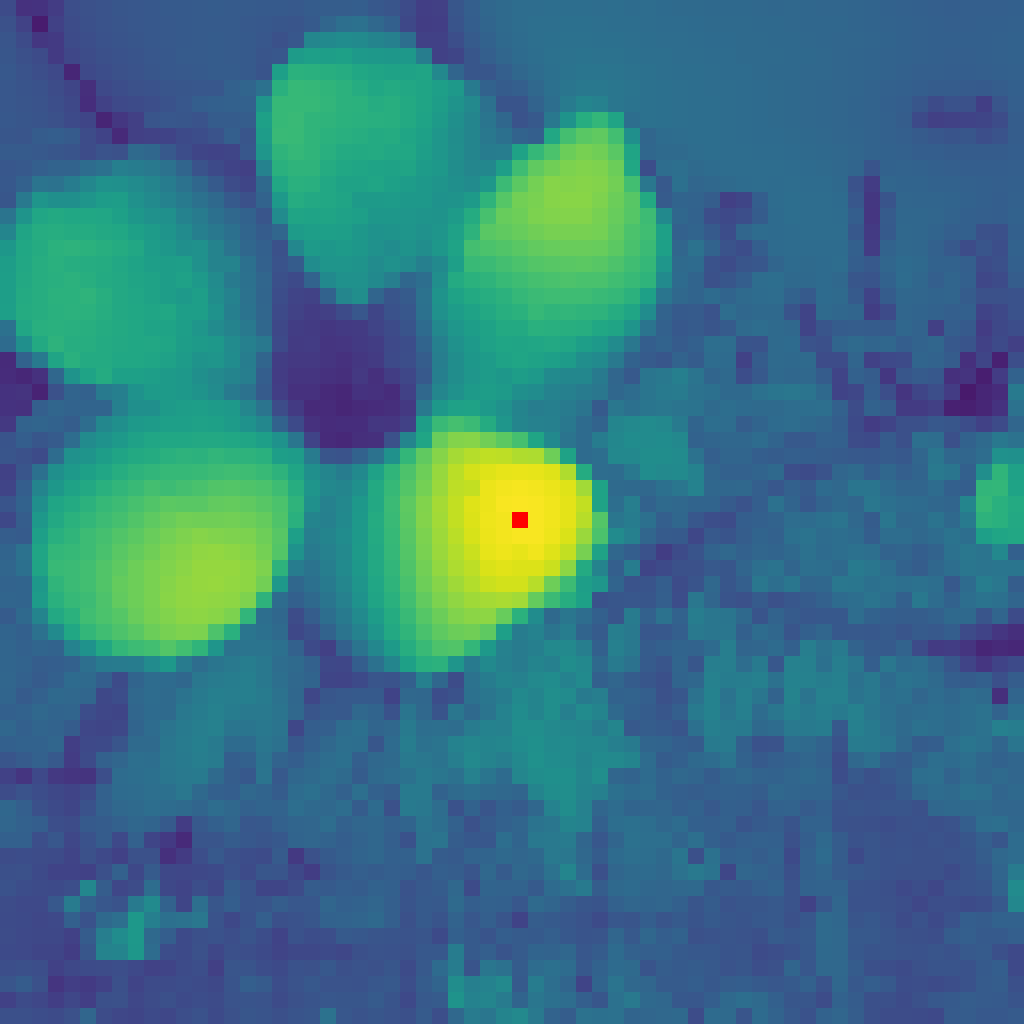
\includegraphics[width=0.19\textwidth]{images/gram/comparison_w_wo/P_20250105_134132.jpg_yolov3_iter9999_1024_seed1_None.png} &
    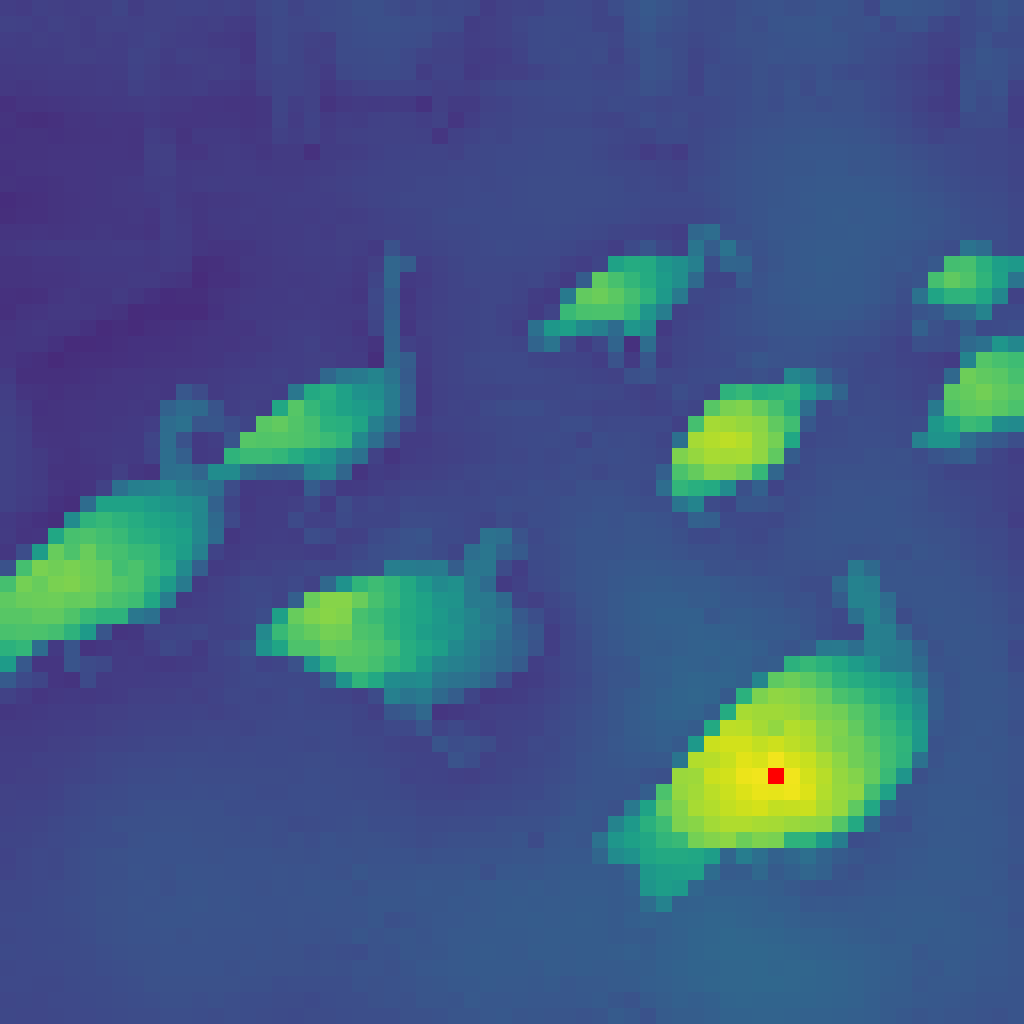
\includegraphics[width=0.19\textwidth]{images/gram/comparison_w_wo/IMG_3727.HEIC_yolov3_iter9999_1024_seed5_None.png} & 
    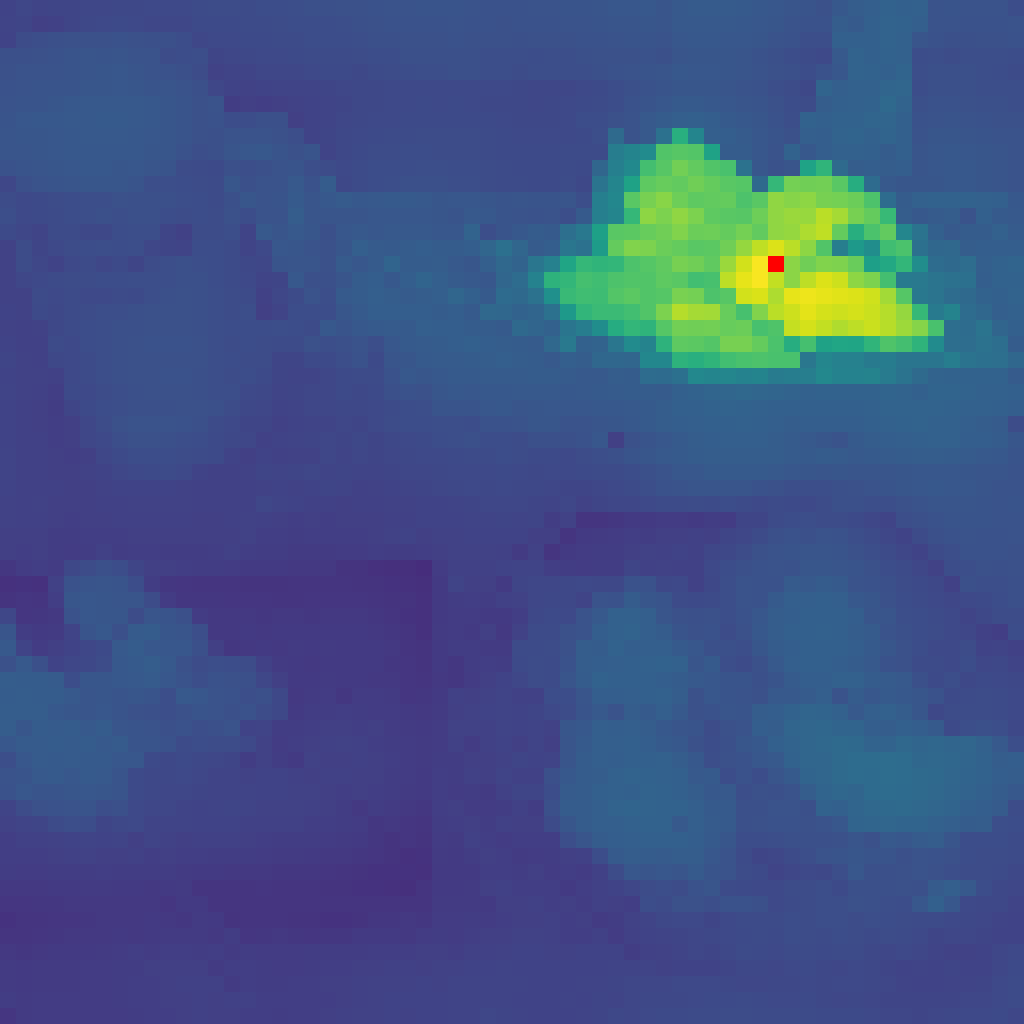
\includegraphics[width=0.19\textwidth]{images/gram/comparison_w_wo/IMG_3730.HEIC_yolov3_iter9999_1024_seed3_None.png} &  
    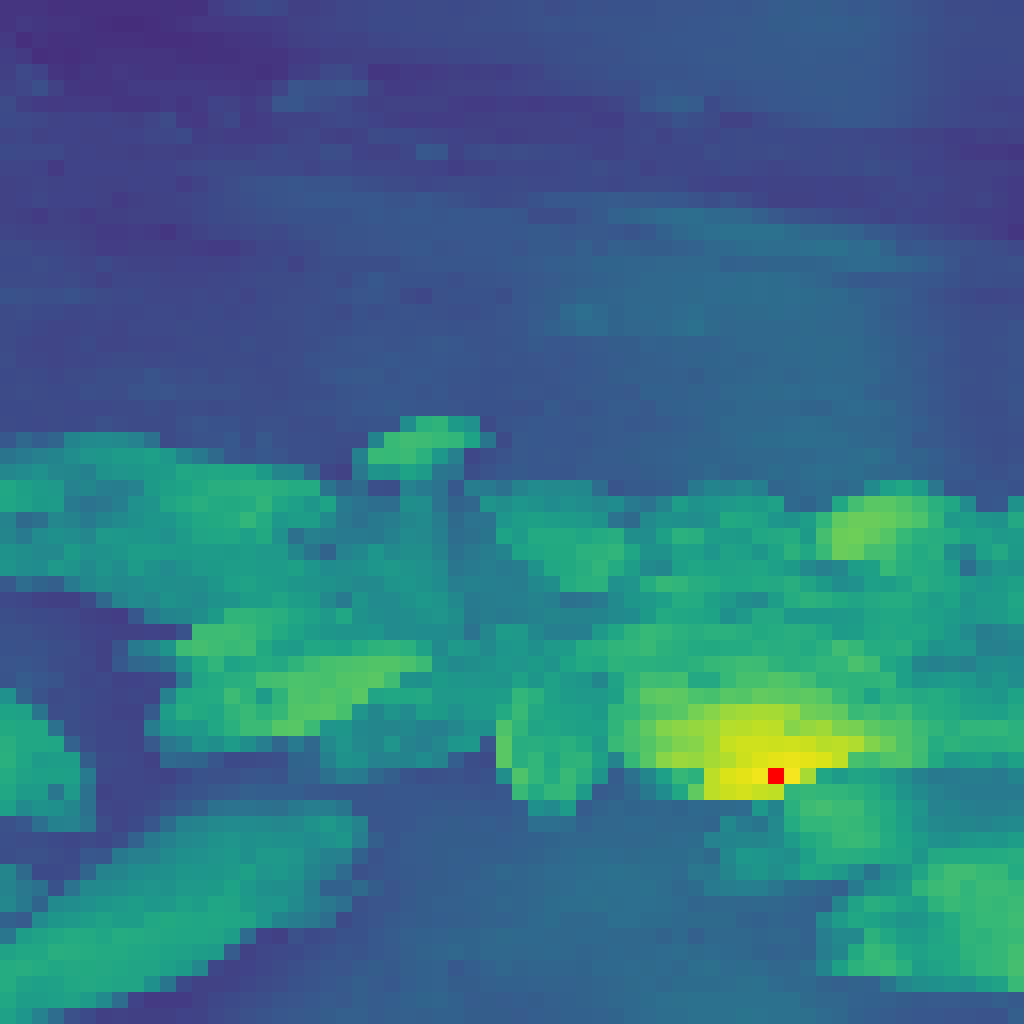
\includegraphics[width=0.19\textwidth]{images/gram/comparison_w_wo/IMG_20190618_192715.jpg_yolov3_iter9999_1024_seed5_None.png} &   
    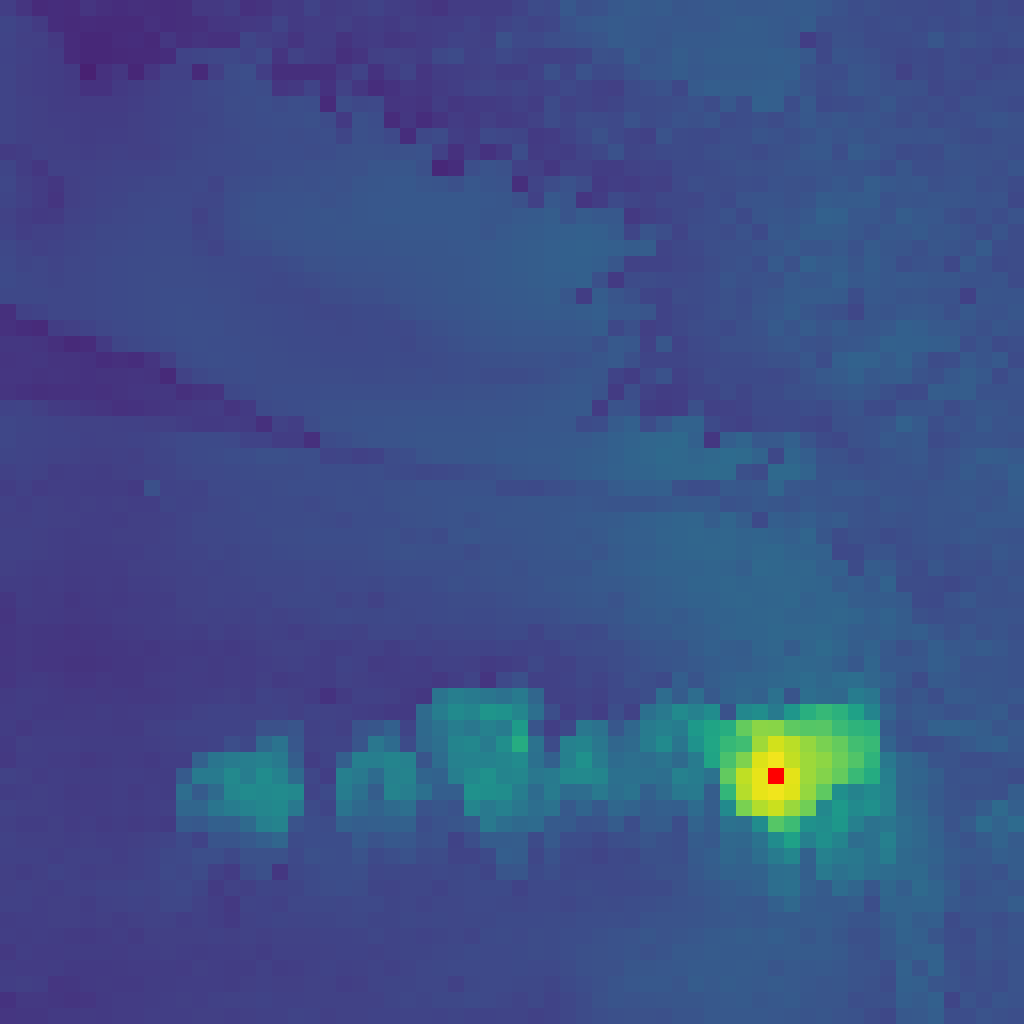
\includegraphics[width=0.19\textwidth]{images/gram/comparison_w_wo/P_20240705_151013.jpg_yolov3_iter9999_1024_seed5_None.png}
    \end{tabular}
    \caption{Qualitative effect of \gramname. We visualize cosine maps before and after using the refinement objective $\mathcal{L}_\mathrm{HRef}$. The input resolution of the images is $1024 \times 1024$ pixels.}
    \label{fig:gram-matrices-comp}
\end{figure}




